% !TEX root = msc_thesis.tex

\mychapter{3}{Results} \label{chap:results}

ELASPIC uses the gradient boosting of decision trees regressor (GBR). It was optimized in several ways.

ELASPIC described in  output xxx features in total.
1. We calculated those features for the Provean and the Skempi training sets.
2. We removed features that were note different in any of the training cases (xxx for core mutations and yyy for interface mutations).

3. It has been reported that balancing the training set by including both positive and negative samples


As described in [], balancing the training set can significantly improve performance. However, with Provean balancing the training set can bias the result because most mutations are to unconserved amino acids (often alanine) and



We built two core predictors and two interface predictors:

\begin{enumerate}
	\item No sequence features but a balanced training set.
	\item Sequence features but no balanced training set.
\end{enumerate}

- Accuracy over different sequence identity bins

- within protein correlation on the test set


\section{Datasets}


\begin{table}[ht]
	\caption[Datasets used in this study.]{Description of the datasets that were used in this study.}
	\label{tab:datasets}
	\begin{tabular}{l | p{9cm} | p{2cm} | p{0.5cm}}
		\toprule
		Name & Description & Type & Ref. \\
		\midrule
		\textbf{Protherm} & Database of changes in the Gibbs free energy of protein folding caused by mutations ($\Delta \Delta G$). & Train & \cite{kumar_protherm_2006} \\
		\textbf{Skempi} & Database of changes in the Gibbs free energy of protein folding caused by mutations ($\Delta \Delta G$). & Train & \cite{moal_skempi:_2012} \\
		\textbf{Taipale} & Chaperone interaction assay measuring protein stability. Change in the interaction with various quality control factors (QCFs), measured using the LUMIER assay. & Validation & \cite{sahni_widespread_2015} \\
		\textbf{Taipale PPI} & Yeast two hybrid studies measuring the effect of mutations on the presence / abscence of interactions. & Validation & \cite{sahni_widespread_2015} \\
		\textbf{Taipale GPCA} & \textit{Gaussia princeps} luciferase protein complementation assay measuring the effect of mutations on protein affinity. & Validation & \cite{sahni_widespread_2015} \\
		\textbf{Humsavar} & Disease-causing mutations vs. polymorphisms. Mostly OMIM, old ClinVar, old COSMIC. $1$ if the mutation is annotated with at least one disease in the UniProt \textit{humsavar.txt} file. $0$ if the mutation is annotated as ``Polymorphism'' in the UniProt \textit{humsavar.txt} file. & Validation \& Test & \cite{consortium_uniprot:_2015} \\
		\textbf{ClinVar} & Disease-causing mutations with a weaker inheritence link than OMIM. $1$ if the mutation is found in the ClinVar \textit{clinvar\_20160531.vcf} file. $0$ if the mutation is found in the ClinVar \textit{common\_no\_known\_medical\_impact\_20160531.vcf} file. & Validation \& Test & \cite{landrum_clinvar:_2016} \\
		\textbf{COSMIC} & Mutations found in cancers. Use high-confidence FATHMM predictions. $1$ if the mutation is predicted to be deleterious by FATHMM in the COSMIC database. $0$ if the mutation is predicted to be benign by FATHMM in the COSMIC database. & Validation \& Test & \cite{forbes_cosmic:_2015} \\
		\textbf{SUMO} & Mutations affecting the activity of SUMO ligase, measured using a cell viability assey. & Test & \cite{cagi4_sumo_ligase} \\
		\textbf{AB-Bind} & Antibody affinity maturation experiments. & Test & \cite{sirin_ab-bind:_2016} \\
		\textbf{Benedix} & Alanine scanning of the TEM1 ($\beta$-lactamase) -- BLIP ($\beta$-lactamase-inhibitor) complex. & Test & \cite{benedix_predicting_2009} \\
	\end{tabular}
\end{table}


\begin{figure}[ht!]
	\centering
	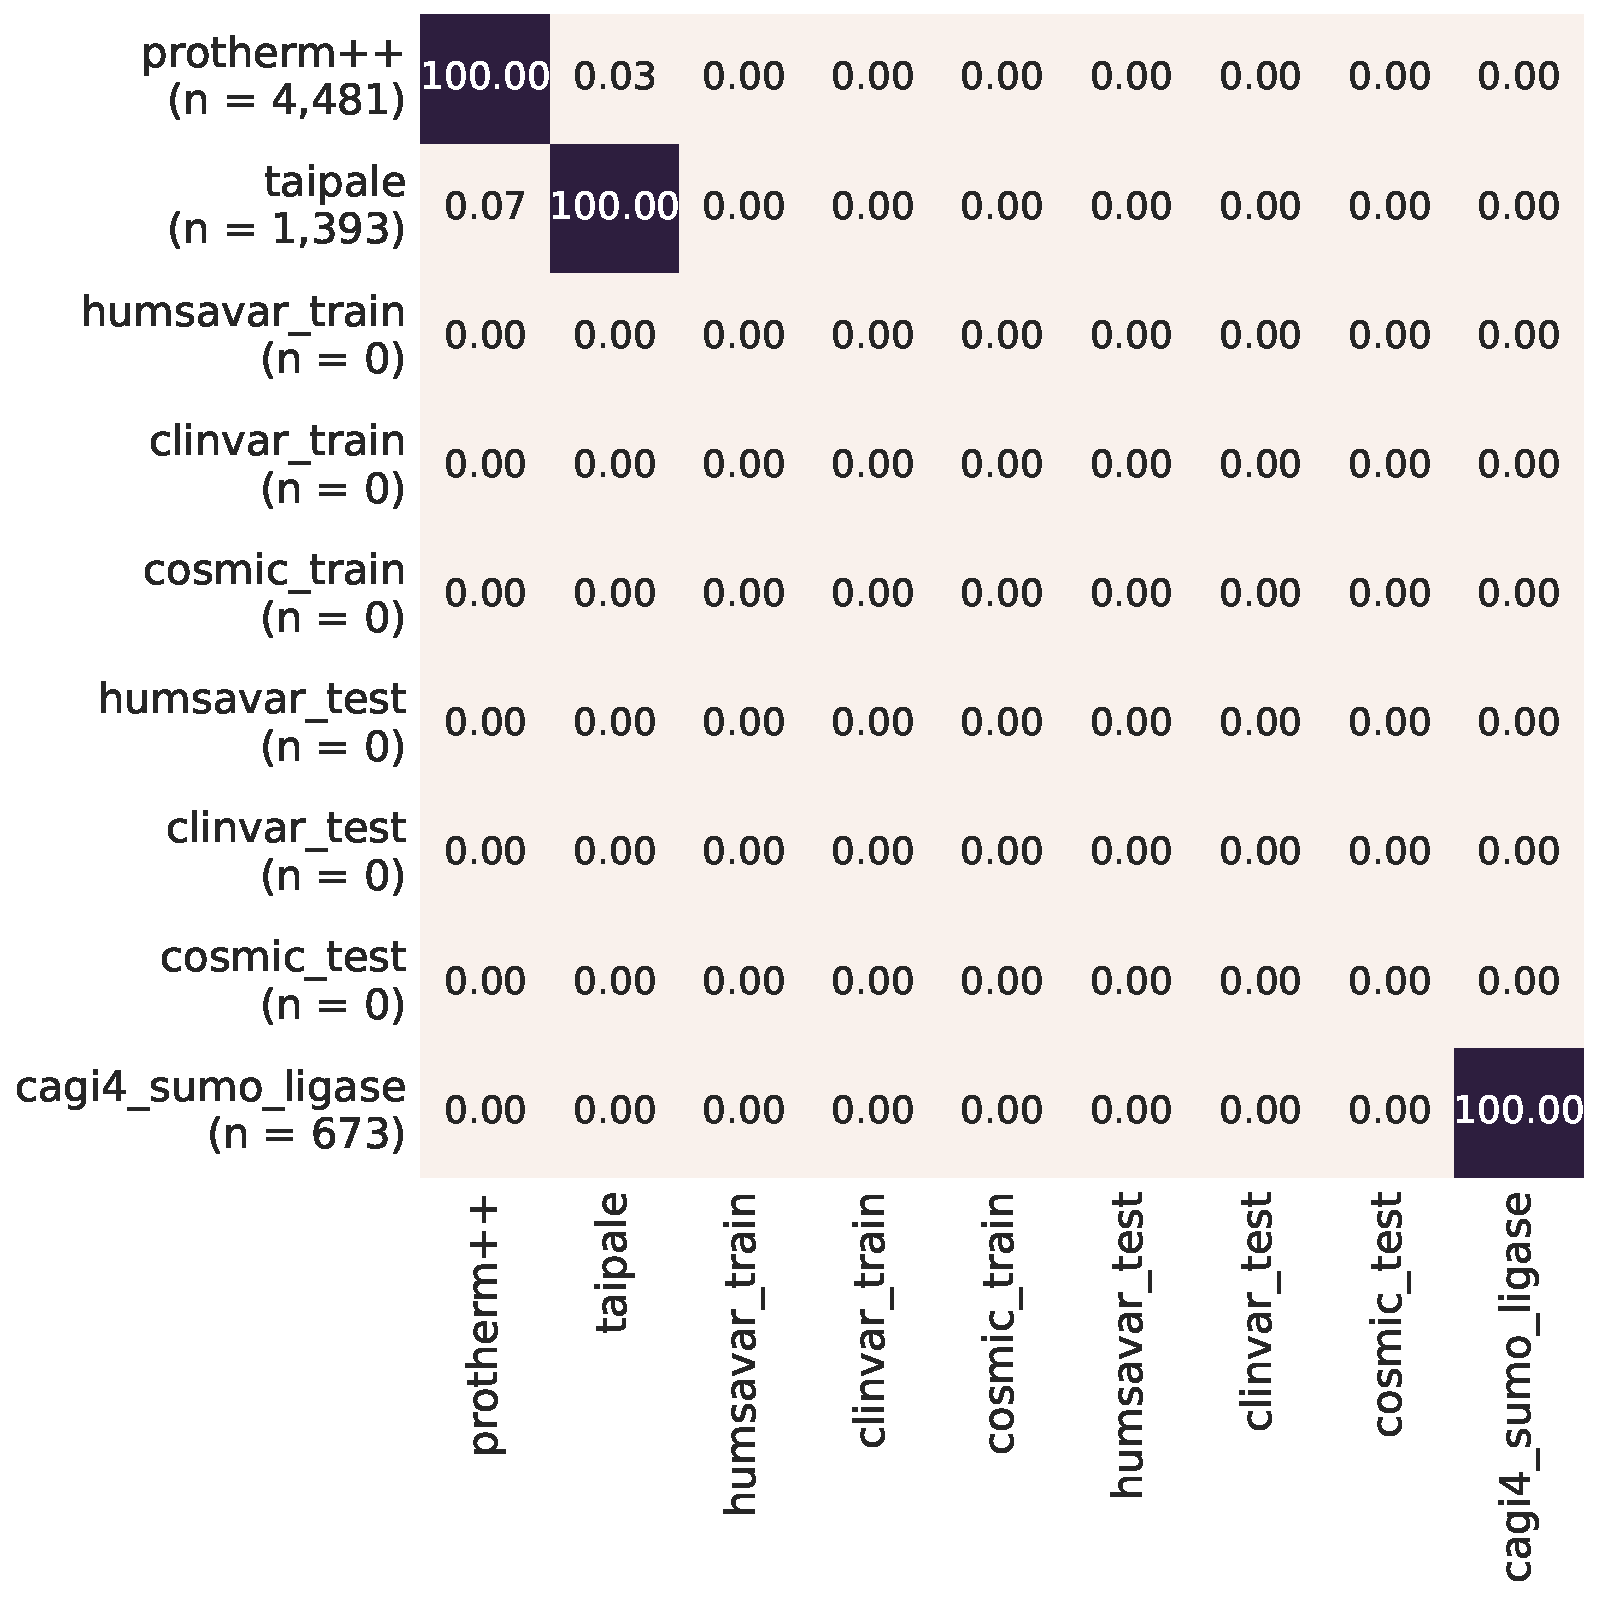
\includegraphics[width=0.65\textwidth]{static/elaspic_training_set/data_statistics/training_set_overlap_data_df_core.pdf}
	\caption[Size and overlap of core and interface datasets.]{Size and overlap of core and interface datasets.}
\end{figure}



\section{Predicting mutation induced $\Delta \Delta G$ of protein folding.}

\begin{figure}[ht!]
	\centering
	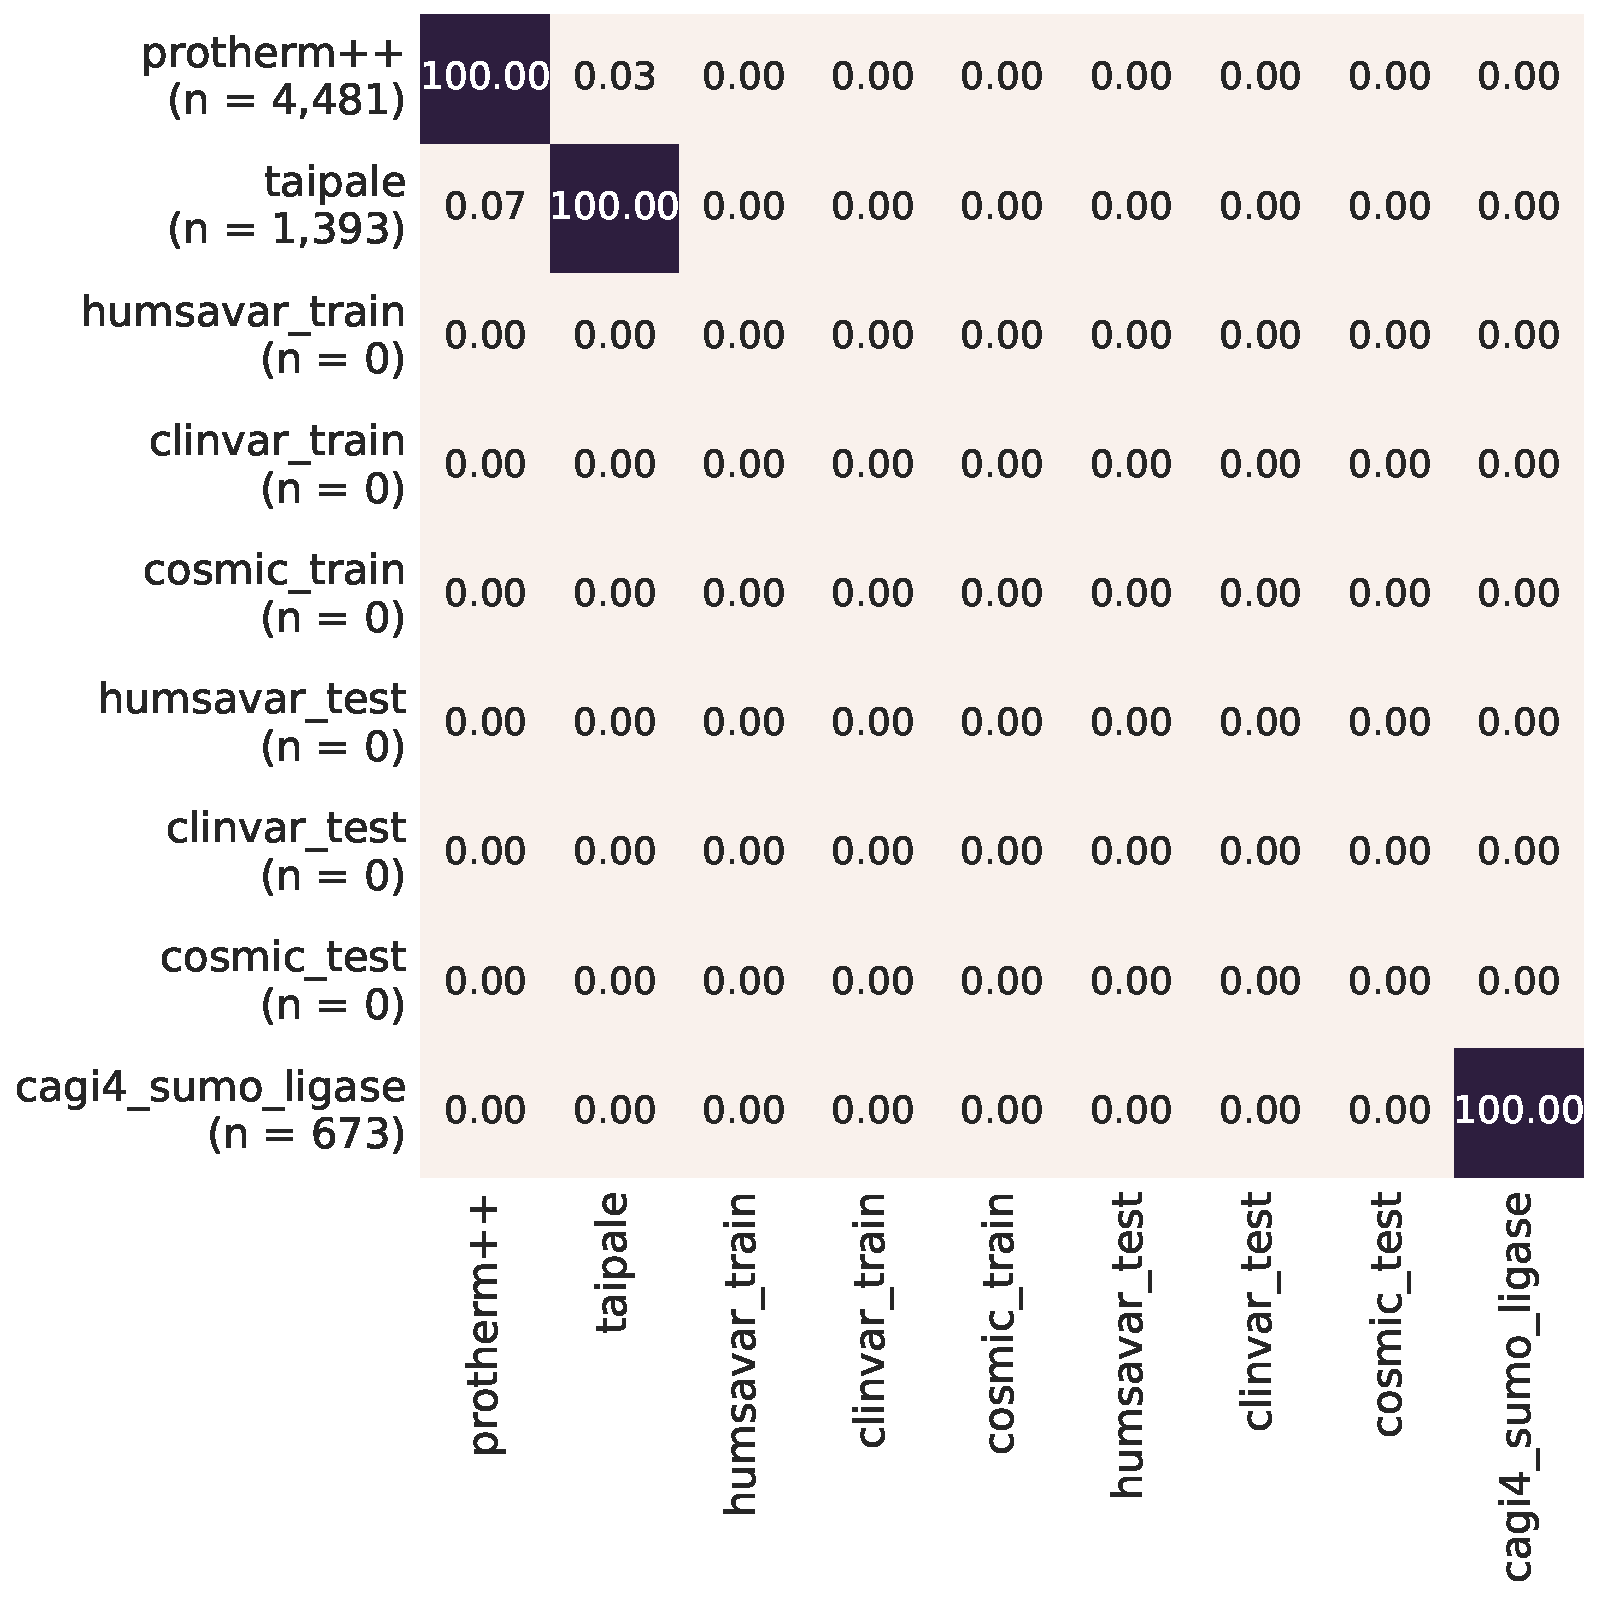
\includegraphics[width=0.65\textwidth]{static/elaspic_training_set/data_statistics/training_set_overlap_data_df_core.pdf}
	\caption[Core predictor datasets.]{Size and overlap of core and interface datasets.}
\end{figure}


\subsection{Gridsearch and feature elimination}

\begin{figure}[ht]
	\centering

	\begin{subfigure}[b]{1.0\textwidth}
		\centering
		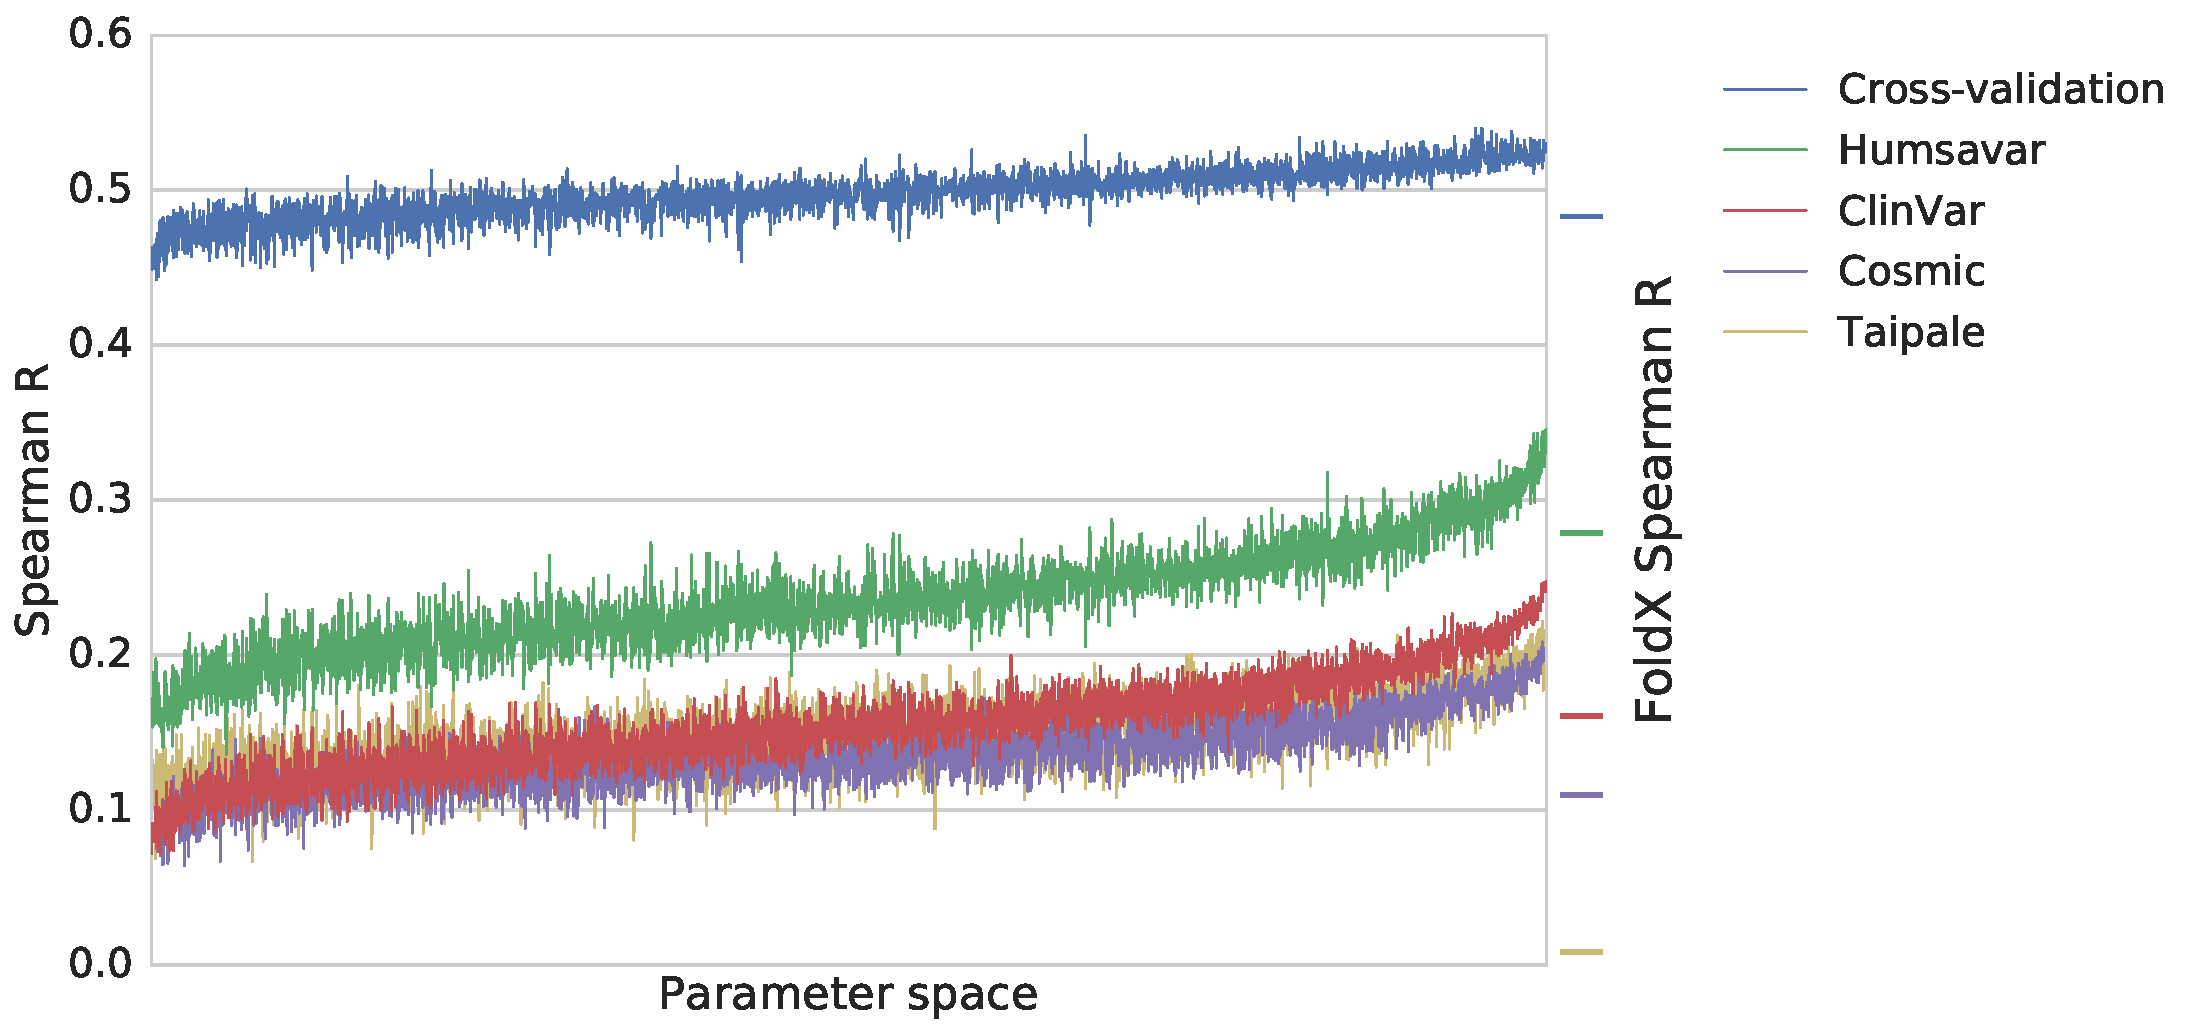
\includegraphics[width=0.6\linewidth]{static/elaspic_training_set/machine_learning/gridsearch_core.pdf}
		\caption{Grid-search over parameter space for the ELASPIC core predictor.}
		\label{fig:gridsearch_core}
	\end{subfigure}

	\begin{subfigure}[b]{1\textwidth}
		\centering
		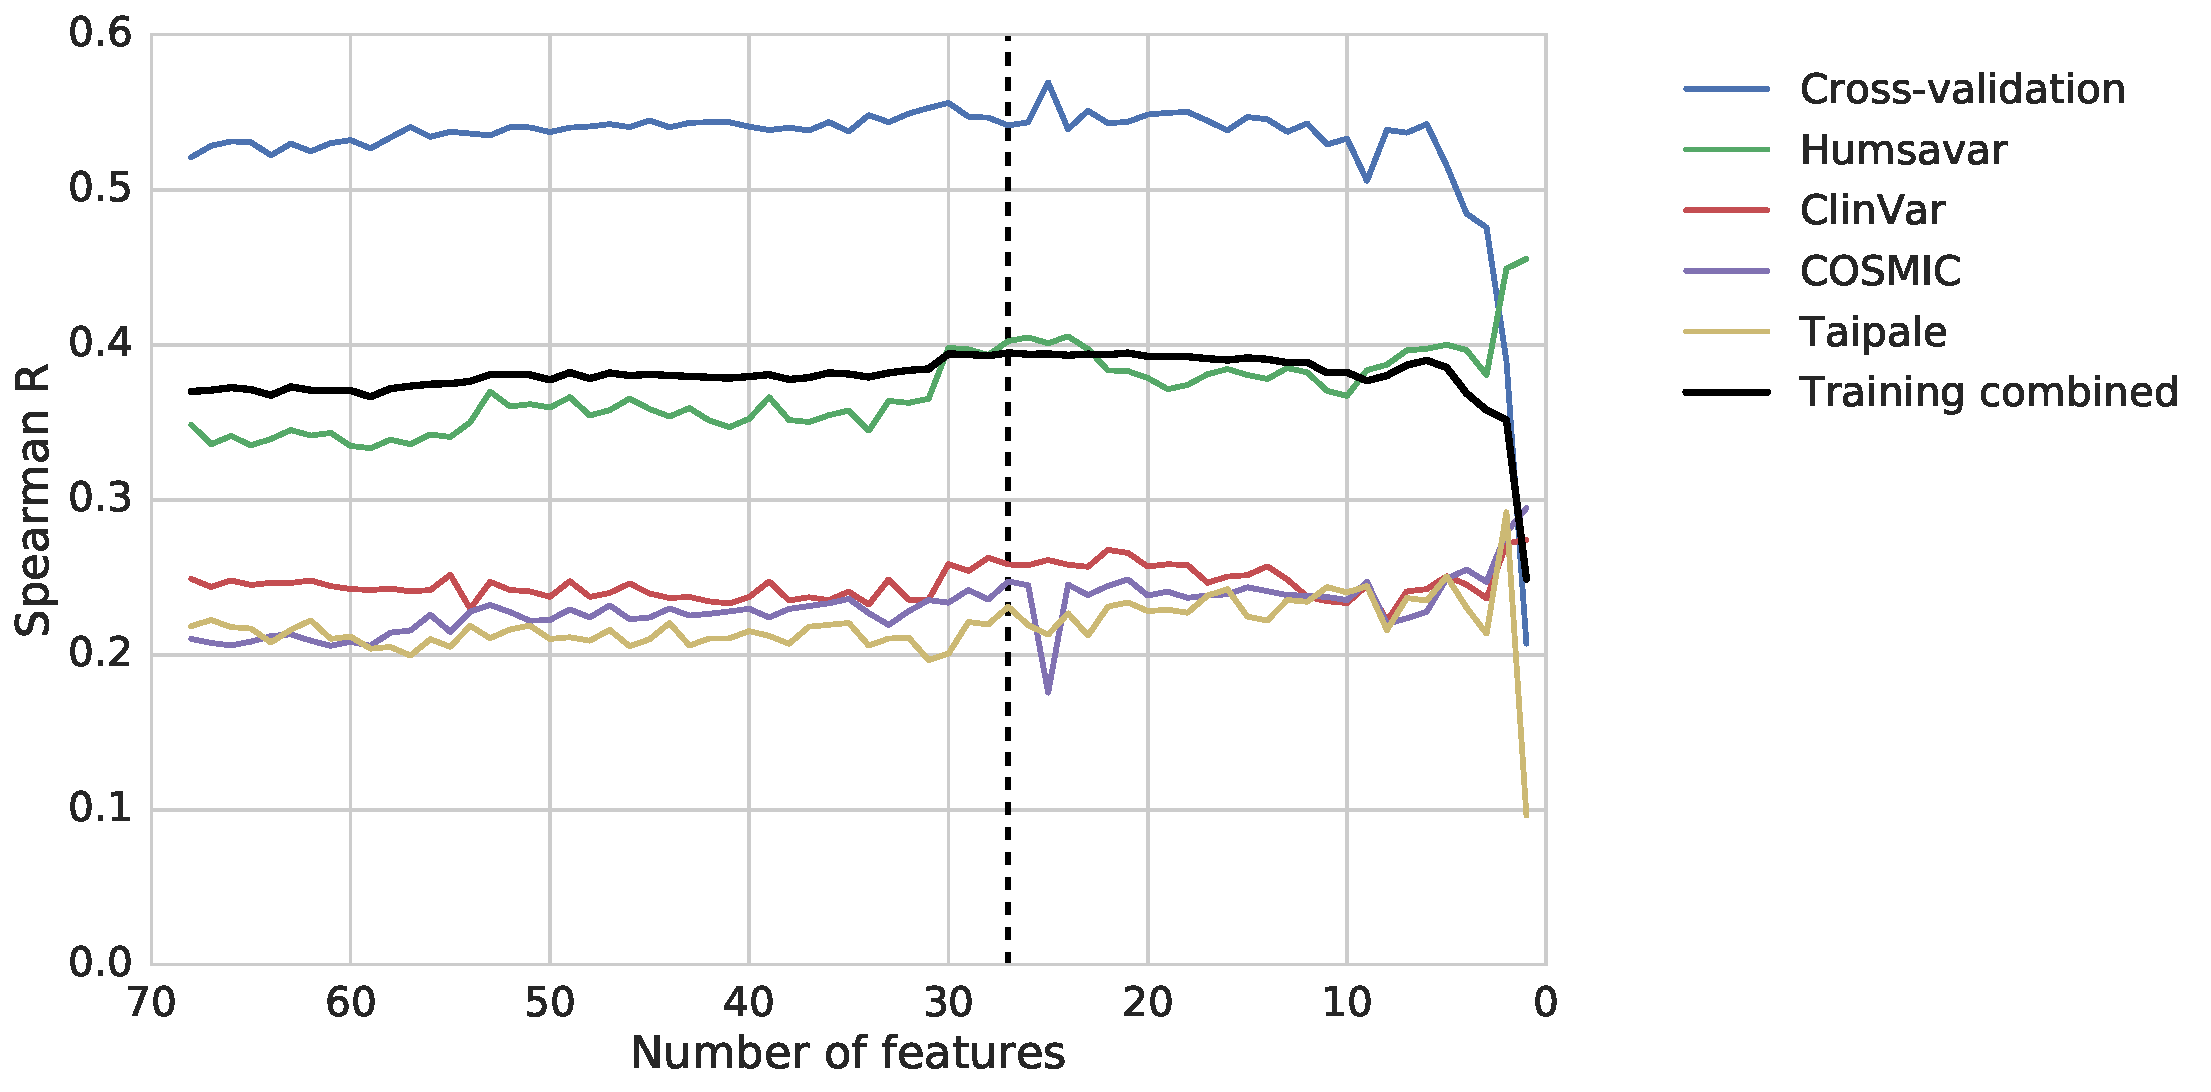
\includegraphics[width=0.75\linewidth]{static/elaspic_training_set/machine_learning/feature_elimination_core.pdf}
		\caption{Feature elimination curve for the ELASPIC core predictor.}
		\label{fig:feature_elimination_core}
	\end{subfigure}

	\caption[Core predictor training.]{Training the core predictor.}
\end{figure}

% Final results

\begin{table}[ht]
\caption{Core predictor parameters.} \label{tab:core_parameters}
\begin{tabular}{l | l | l}
	\toprule
	Parameter label & Parameter description & Parameter value \\
	\midrule
	... & ... \\
	\bottomrule
\end{tabular}
\end{table}


\begin{table}[ht]
	\caption{Core predictor features.} \label{tab:core_features}
	\begin{tabular}{ | l | l | l | l | }
	\hline
		alignment\_coverage & Alignment quality & \  & \  \\ \hline
		alignment\_identity & Alignment quality & \  & \  \\ \hline
		alignment\_score & Alignment quality & \  & \  \\ \hline
		backbone\_hbond\_change & FoldX & \  & \  \\ \hline
		backbone\_hbond\_wt & FoldX & \  & \  \\ \hline
		cis\_bond\_wt & FoldX & \  & \  \\ \hline
		disulfide\_wt & FoldX & \  & \  \\ \hline
		electrostatic\_kon\_change & FoldX & \  & \  \\ \hline
		electrostatics\_change & FoldX & * & \  \\ \hline
		entropy\_mainchain\_change & FoldX & \  & \  \\ \hline
		helix\_dipole\_wt & FoldX & \  & \  \\ \hline
		matrix\_score & Sequence conservation & \  & \  \\ \hline
		pcv\_hbond\_change & Physico-chemical features & \  & \  \\ \hline
		pcv\_hbond\_self\_change & Physico-chemical features & \  & \  \\ \hline
		pcv\_salt\_equal\_change & Physico-chemical features & \  & \  \\ \hline
		pcv\_salt\_equal\_self\_wt & Physico-chemical features & \  & \  \\ \hline
		pcv\_salt\_equal\_wt & Physico-chemical features & \  & \  \\ \hline
		pcv\_salt\_opposite\_change & Physico-chemical features & \  & \  \\ \hline
		pcv\_vdw\_self\_change & Physico-chemical features & \  & \  \\ \hline
		provean\_score & Sequence conservation & ** &  \\ \hline
		sloop\_entropy\_wt & FoldX & \  & \  \\ \hline
		solvation\_hydrophobic\_change & FoldX & * & \  \\ \hline
		solvation\_polar\_change & FoldX & ** &  \\ \hline
		solvent\_accessibility\_wt & FoldX & * & \  \\ \hline
		torsional\_clash\_change & FoldX & \  & \  \\ \hline
		van\_der\_waals\_clashes\_change & FoldX & * & \  \\ \hline
		water\_bridge\_wt & FoldX & \  & \  \\ \hline
	\end{tabular}
\end{table}


\subsection{Validation}

\begin{figure}[ht]
	% \centering

	\begin{subfigure}[b]{1.0\textwidth}
		\centering
		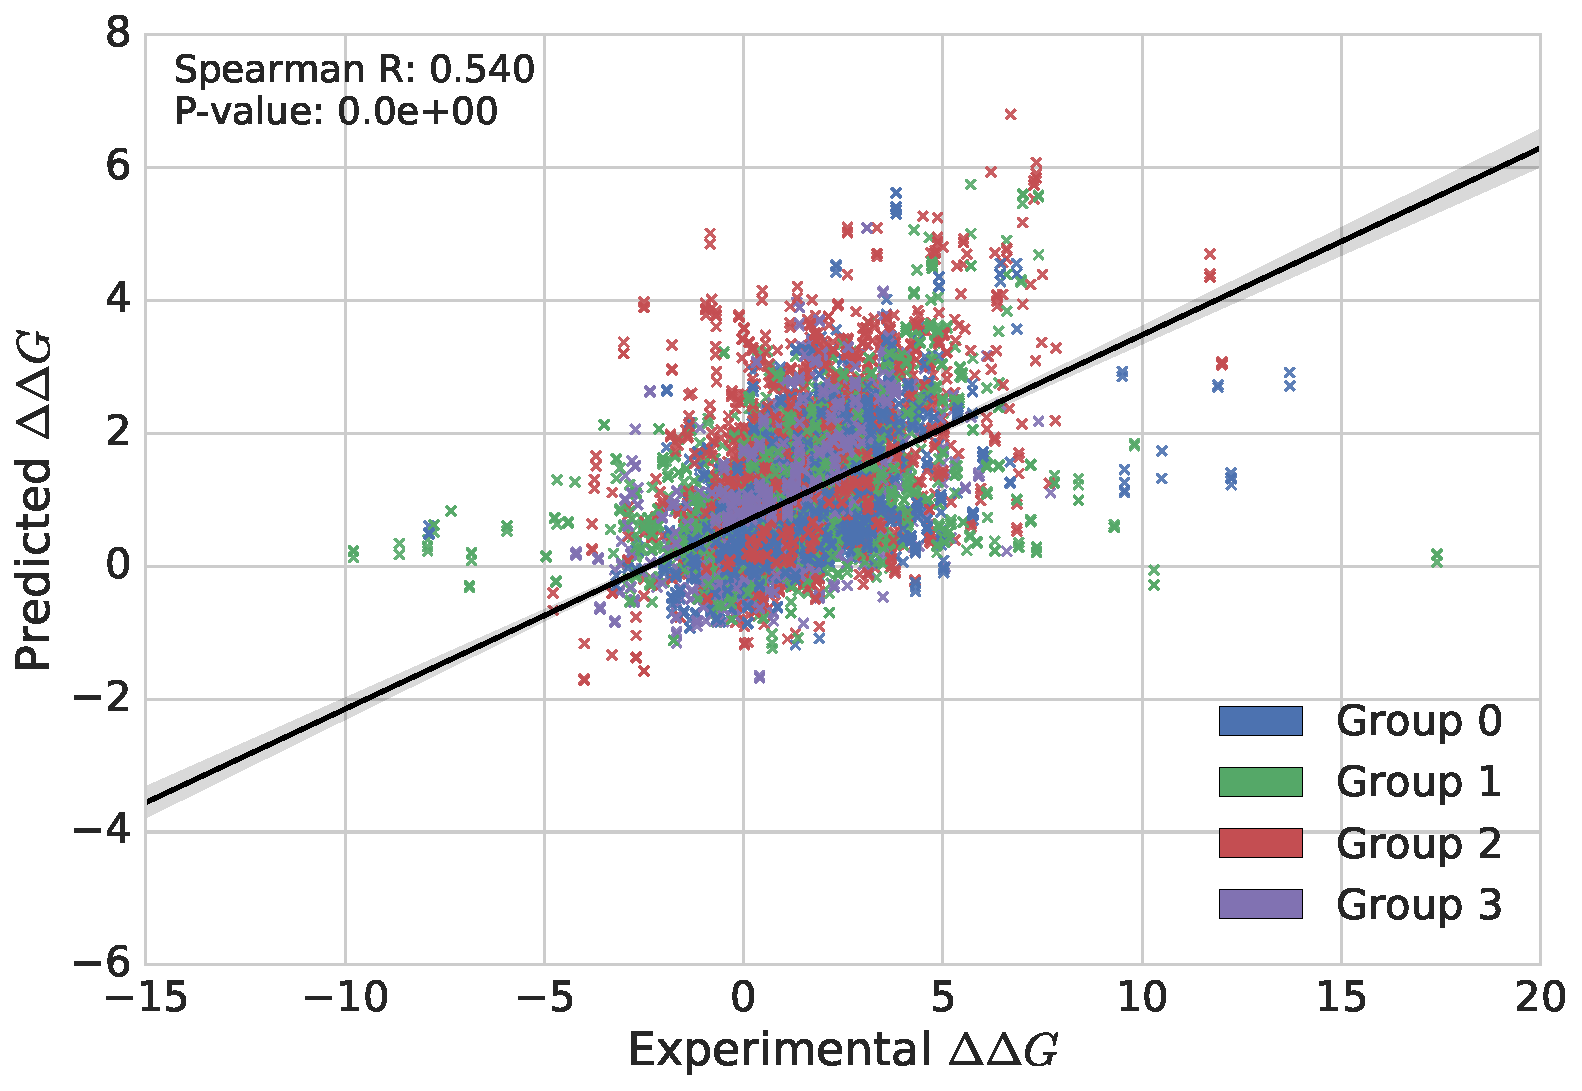
\includegraphics[width=0.6\linewidth]{static/elaspic_training_set/validation/crossvalidation_performance_core.pdf}
		\caption{Four-fold cross-validation performance on the training dataset. Colors indicate cross-validation bins.}
		\vspace*{10mm}
	\end{subfigure}

	\begin{subfigure}[b]{1.0\textwidth}
		\centering
		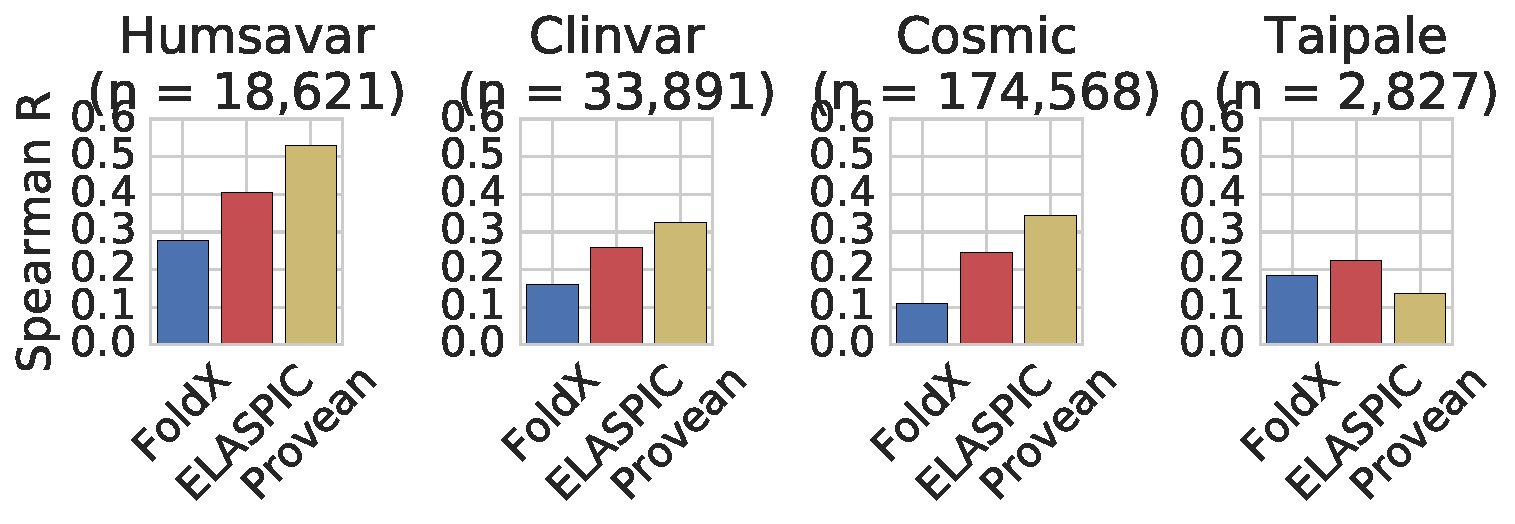
\includegraphics[width=0.8\textwidth]{static/elaspic_training_set/validation/validation_performance_core.pdf}
		\caption{Performance on the validation datasets.}
		\vspace*{10mm}
	\end{subfigure}

	\begin{subfigure}[b]{1.0\textwidth}
		\centering
		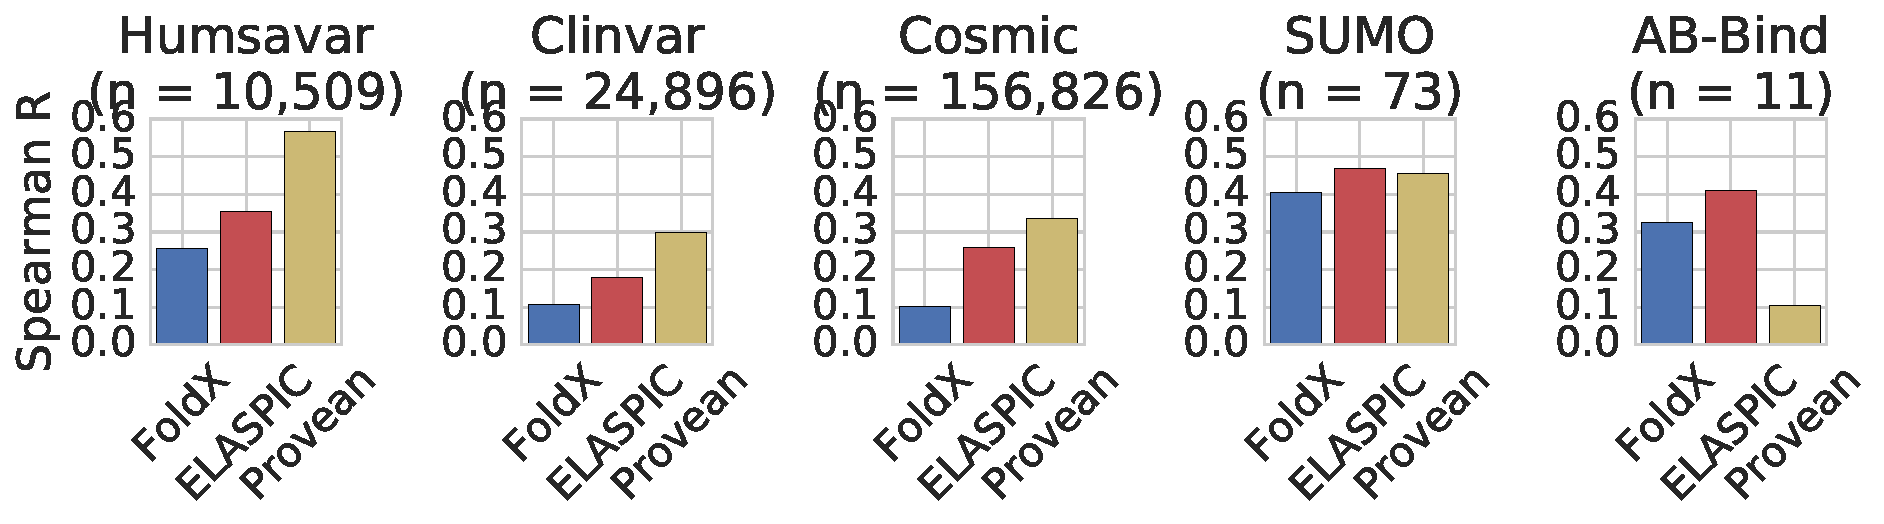
\includegraphics[width=1.0\textwidth]{static/elaspic_training_set/validation/test_performance_core.pdf}
		\caption{Performance on the test datasets.}
		% \vspace*{10mm}
	\end{subfigure}

	\caption[Core predictor validation.]{Performance of the core predictor on the training (a), validation (b) and test sets (c).}
\end{figure}




\section{Predicting mutation induced $\Delta \Delta G$ of protein-protein interactions.}

\begin{figure}[ht]
	\centering
	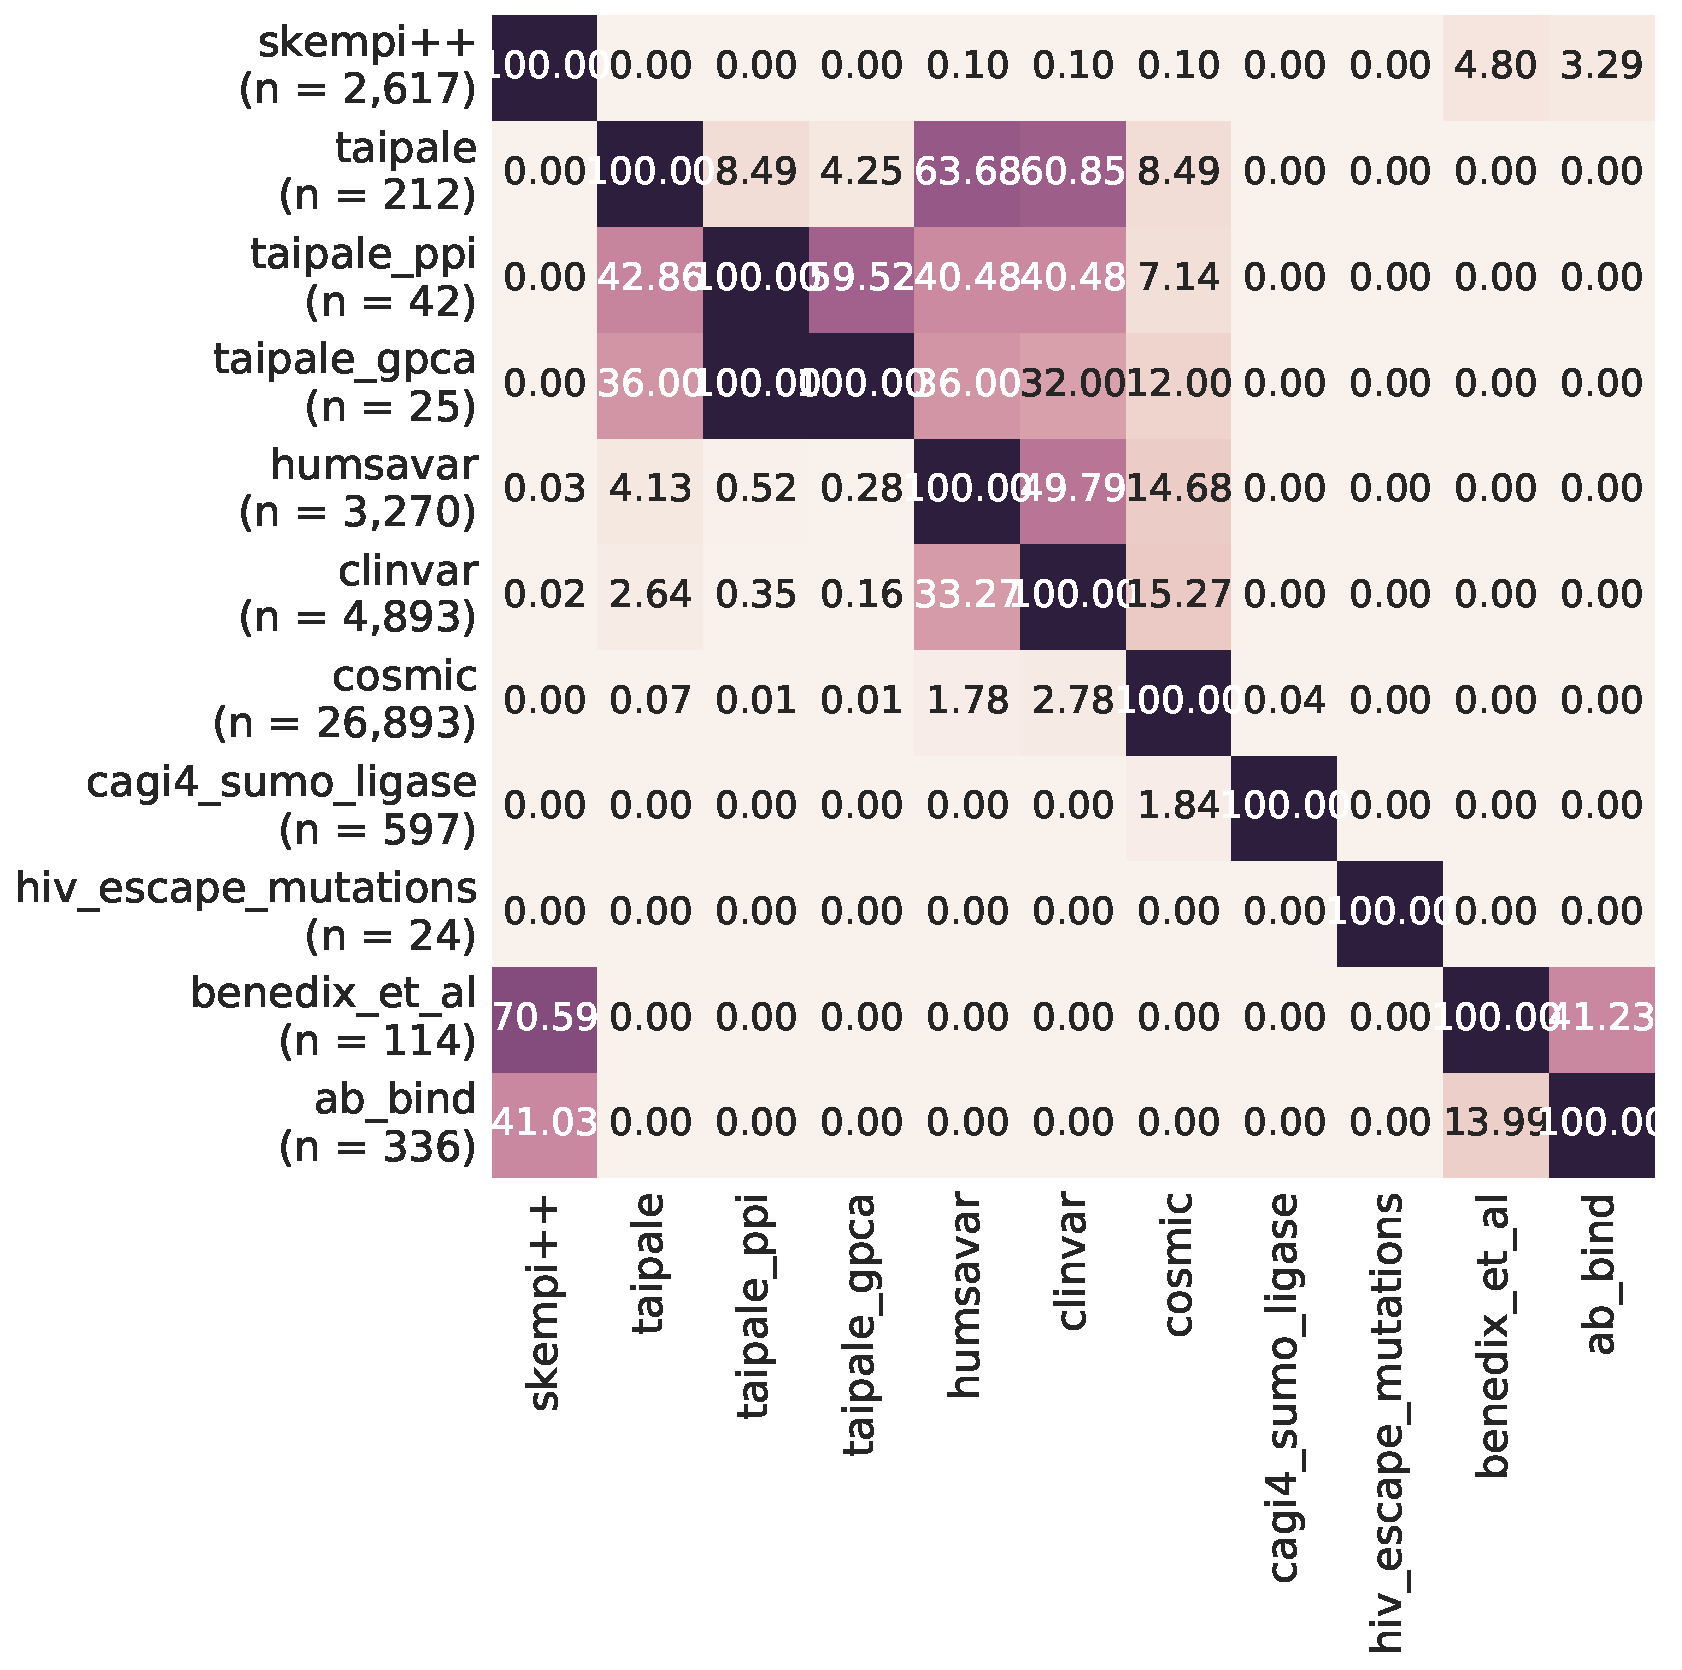
\includegraphics[width=0.65\textwidth]{static/elaspic_training_set/data_statistics/training_set_overlap_data_df_interface.pdf}
	\caption[Interface predictor datasets.]{Size and overlap between the core and interface predictor datasets.}
\end{figure}


\subsection{Gridsearch and feature elimination}

\begin{figure}[ht]
	\centering

	\begin{subfigure}[b]{1.0\textwidth}
		\centering
		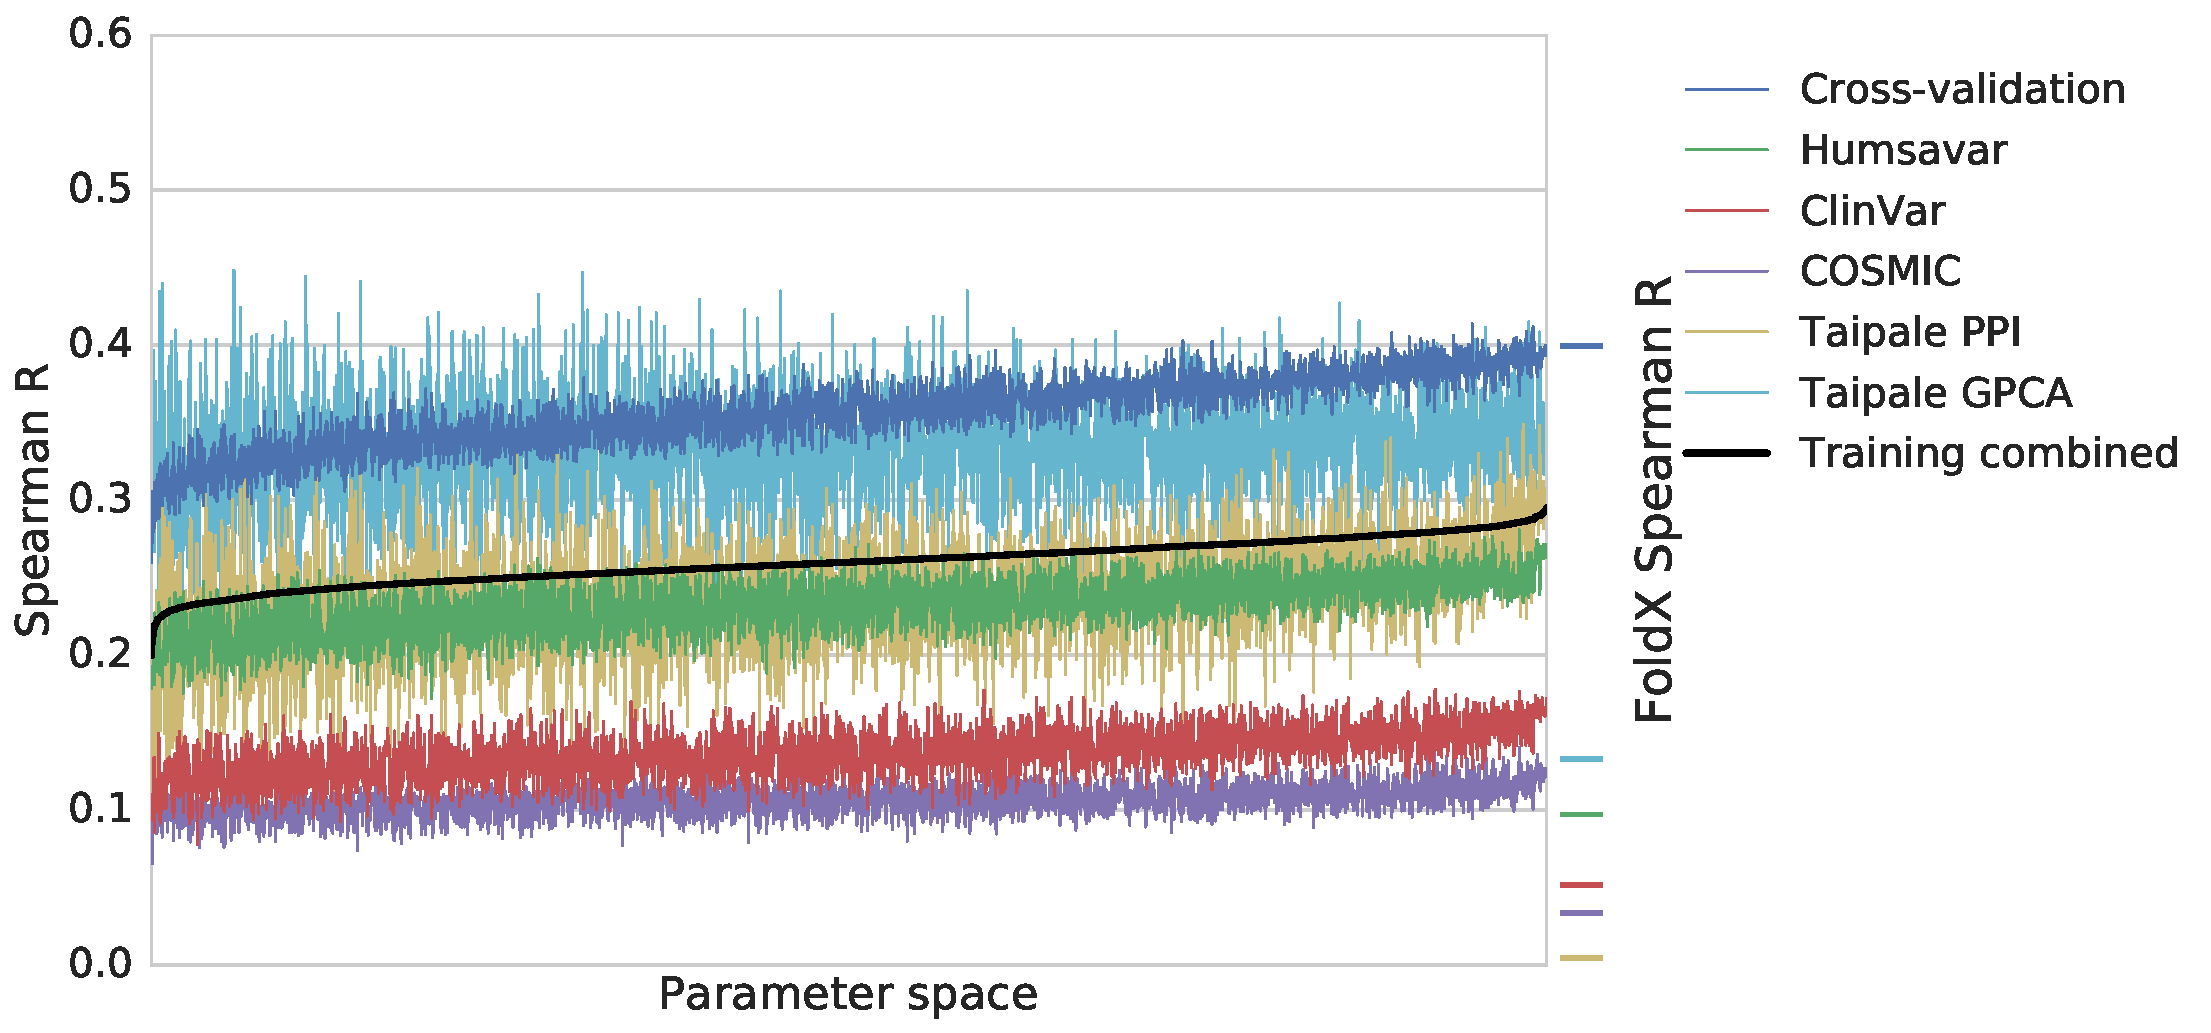
\includegraphics[width=0.6\linewidth]{static/elaspic_training_set/machine_learning/gridsearch_interface.pdf}
		\caption{Grid-search over parameter space.}
		\label{fig:gridsearch_interface}
	\end{subfigure}

	\begin{subfigure}[b]{1\textwidth}
		\centering
		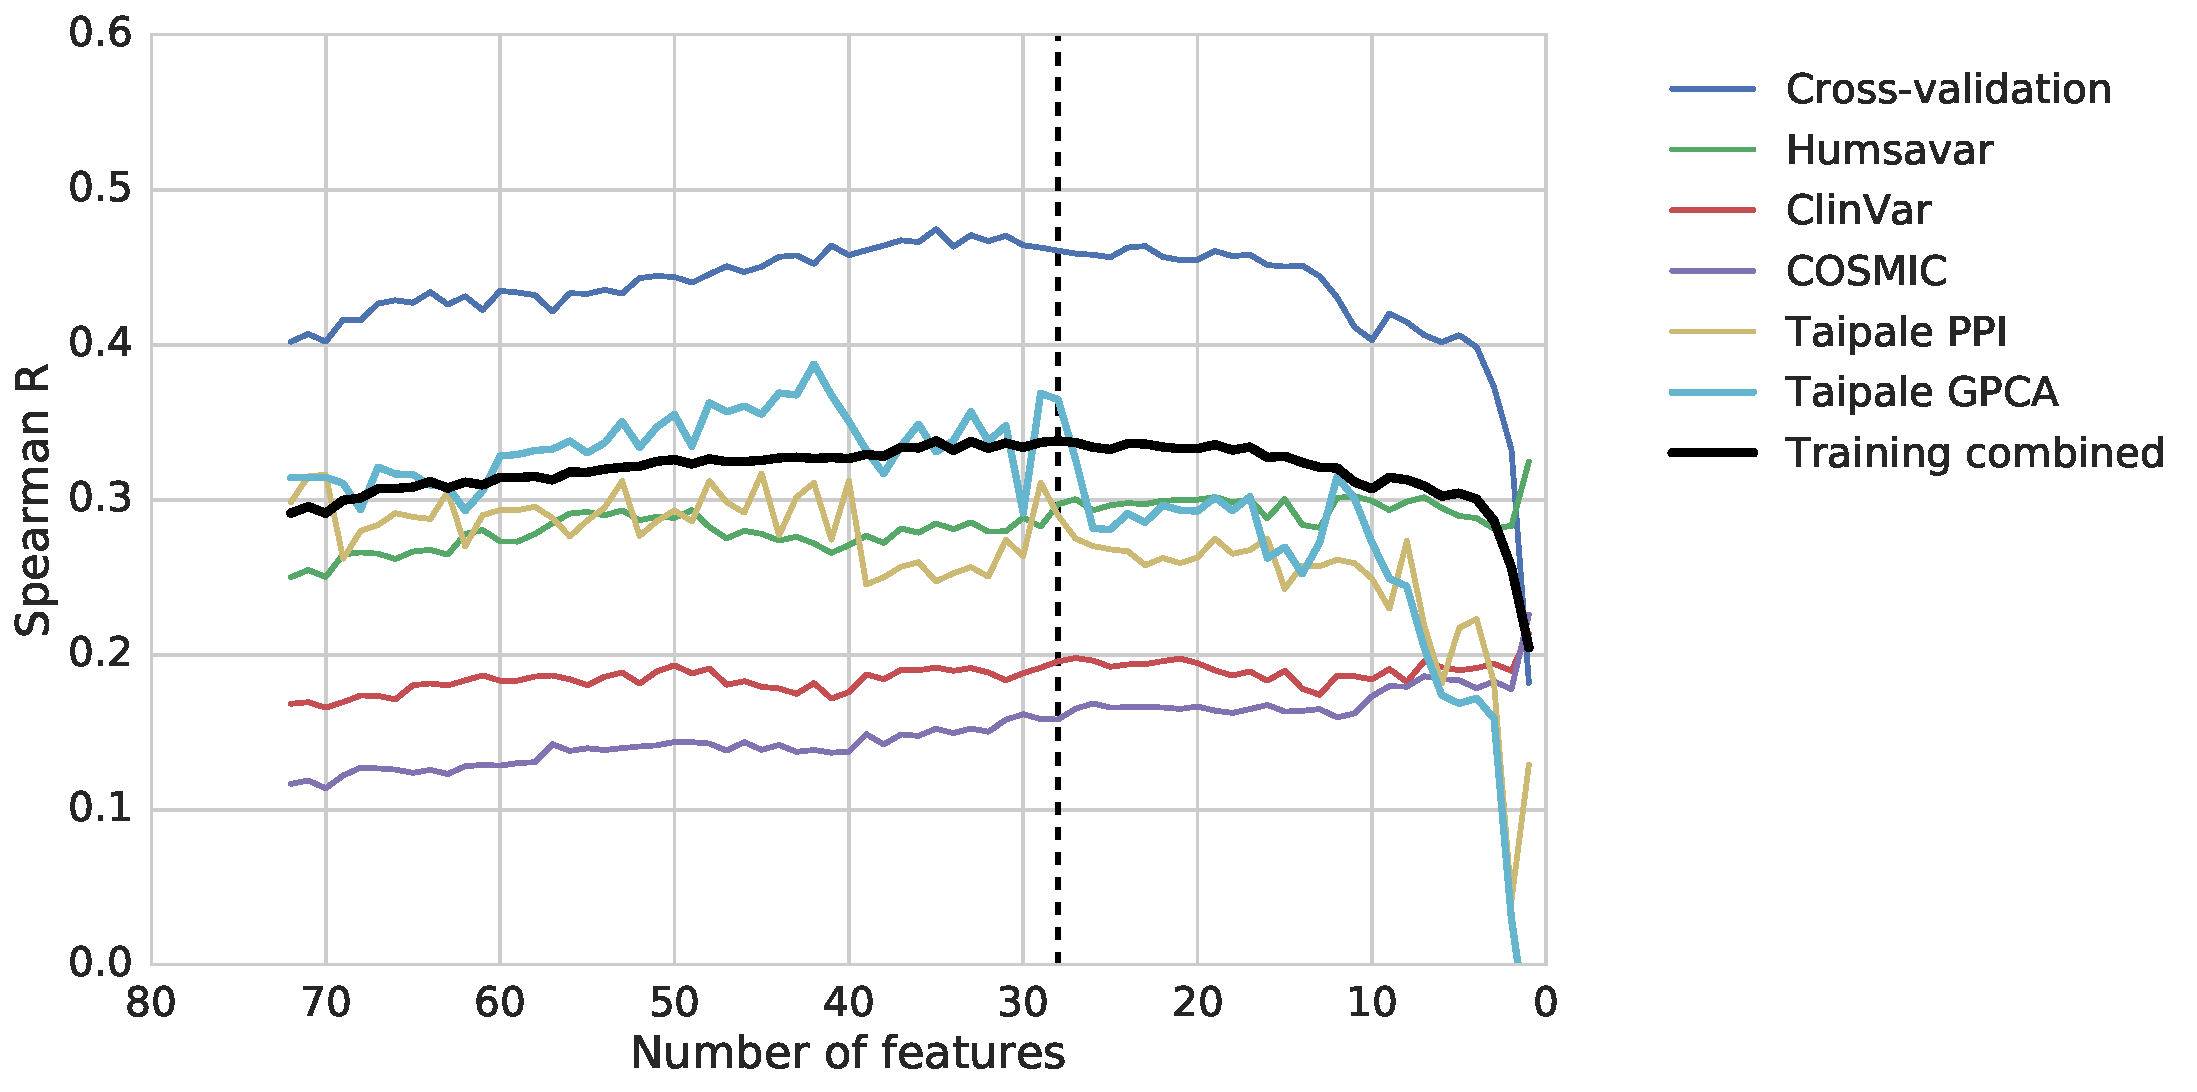
\includegraphics[width=0.75\linewidth]{static/elaspic_training_set/machine_learning/feature_elimination_interface.pdf}
		\caption{Feature elimination.}
		\label{fig:feature_elimination_interface}
	\end{subfigure}

	\caption[Interface predictor training.]{Training the interface predictor.}
\end{figure}


% Final results

\begin{table}[ht]
\caption{Interface predictor parameters.} \label{tab:interface_parameters}
\begin{tabular}{l | l | l}
	\toprule
	Parameter label & Parameter description & Parameter value \\
	\midrule
	... & ... \\
	\bottomrule
\end{tabular}
\end{table}


\begin{table}[ht]
\caption{Interface predictor features.} \label{tab:interface_features}
	\begin{tabular}{ | l | l | l | }
	Feature name & Feature description & ... \\
	\hline
		alignment\_score & Alignment quality & \  \\ \hline
		backbone\_clash\_change & FoldX & \  \\ \hline
		backbone\_clash\_wt & FoldX & \  \\ \hline
		backbone\_hbond\_change & FoldX & \  \\ \hline
		cis\_bond\_wt & FoldX & \  \\ \hline
		electrostatic\_kon\_wt & FoldX & \  \\ \hline
		energy\_ionisation\_wt & FoldX & \  \\ \hline
		entropy\_complex\_change & FoldX & \  \\ \hline
		entropy\_sidechain\_change & FoldX & * \\ \hline
		intraclashes\_energy\_2\_change & FoldX & \  \\ \hline
		partial\_covalent\_bonds\_wt & FoldX & * \\ \hline
		pcv\_hbond\_self\_change & Physico-chemical features & \  \\ \hline
		pcv\_hbond\_wt & Physico-chemical features & \  \\ \hline
		pcv\_salt\_equal\_self\_change & Physico-chemical features & \  \\ \hline
		pcv\_salt\_equal\_wt & Physico-chemical features & \  \\ \hline
		pcv\_salt\_opposite\_change & Physico-chemical features & \  \\ \hline
		pcv\_salt\_opposite\_self\_change & Physico-chemical features & \  \\ \hline
		pcv\_salt\_opposite\_self\_wt & Physico-chemical features & \  \\ \hline
		pcv\_vdw\_self\_change & Physico-chemical features & \  \\ \hline
		pcv\_vdw\_self\_wt & Physico-chemical features & * \\ \hline
		pcv\_vdw\_wt & Physico-chemical features & * \\ \hline
		provean\_score & Sequence conservation & * \\ \hline
		sloop\_entropy\_change & FoldX & \  \\ \hline
		solvation\_hydrophobic\_change & FoldX & \  \\ \hline
		solvation\_polar\_change & FoldX & * \\ \hline
		solvation\_polar\_wt & FoldX & \  \\ \hline
		torsional\_clash\_change & FoldX & \  \\ \hline
		water\_bridge\_change & FoldX & \  \\ \hline
	\end{tabular}
\end{table}


\subsection{Validation}

\begin{figure}[ht]
	% \centering

	\begin{subfigure}[b]{1.0\textwidth}
		\centering
		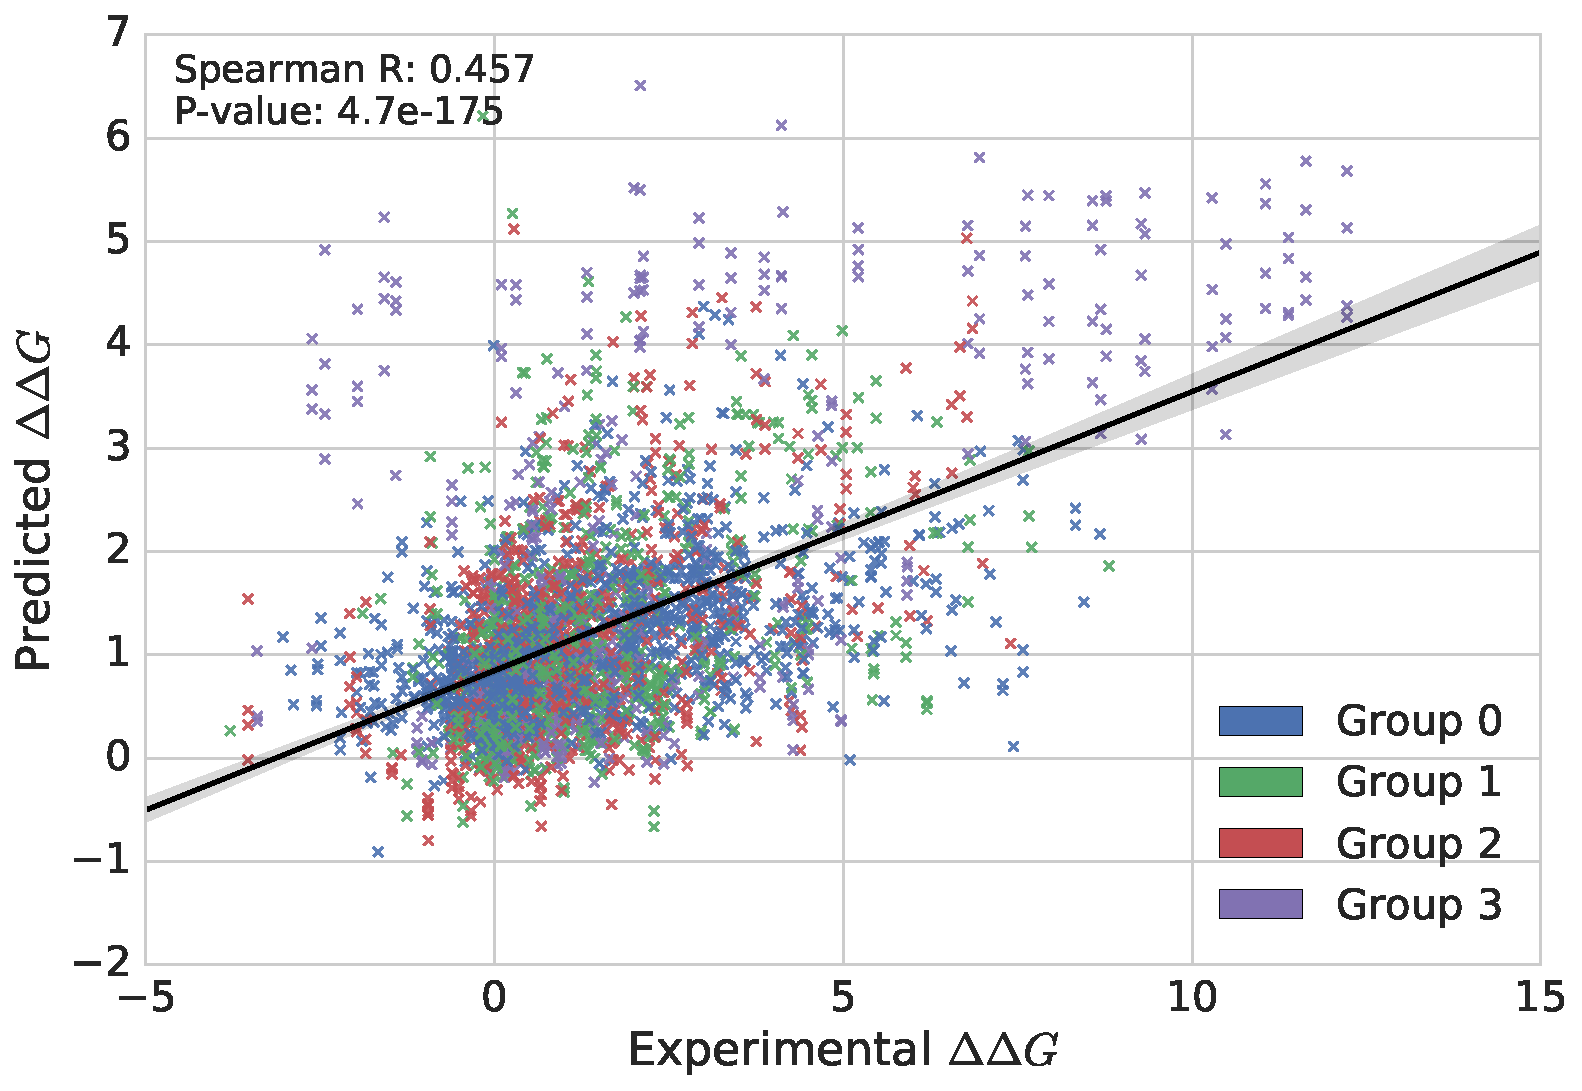
\includegraphics[width=0.6\linewidth]{static/elaspic_training_set/validation/crossvalidation_performance_interface.pdf}
		\caption{Four-fold cross-validation performance on the training dataset. Colors indicate cross-validation bins.}
		\vspace*{10mm}
	\end{subfigure}

	\begin{subfigure}[b]{1.0\textwidth}
		\centering
		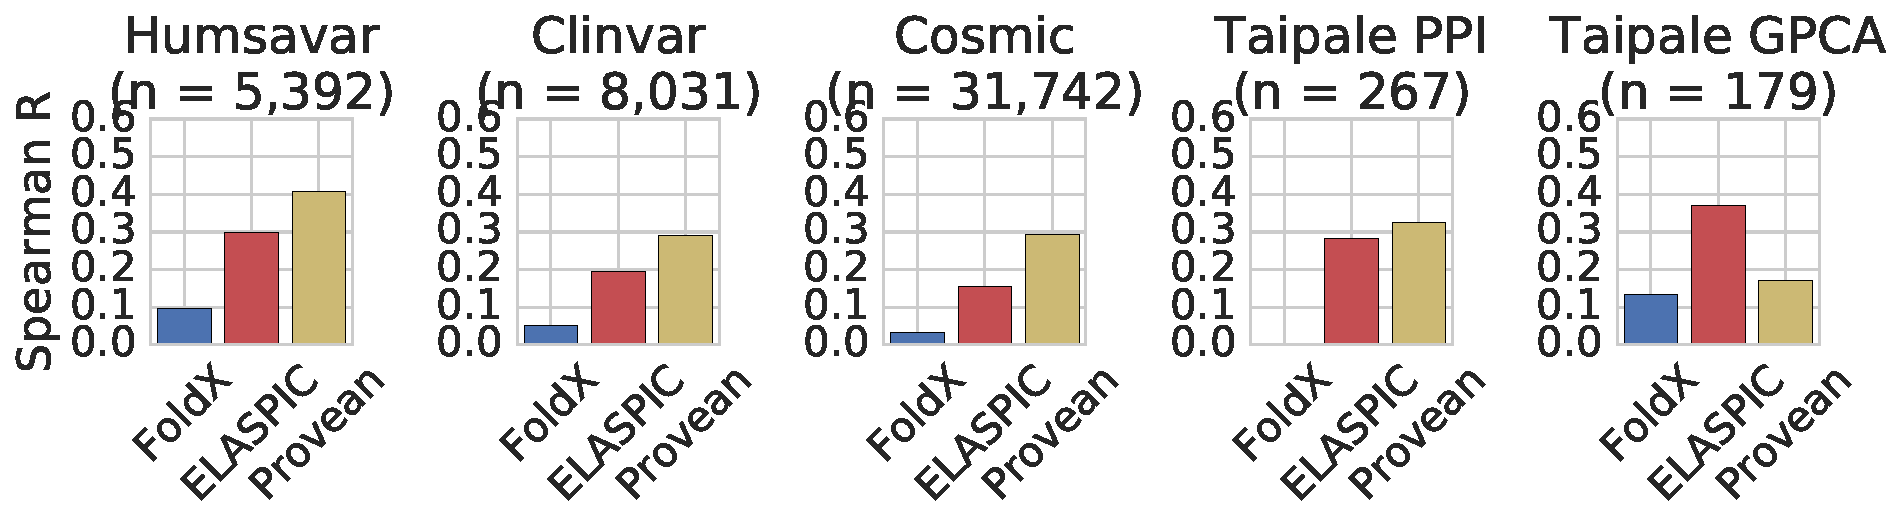
\includegraphics[width=0.8\textwidth]{static/elaspic_training_set/validation/validation_performance_interface.pdf}
		\caption{Performance on the validation datasets.}
		\vspace*{10mm}
	\end{subfigure}

	\begin{subfigure}[b]{1.0\textwidth}
		\centering
		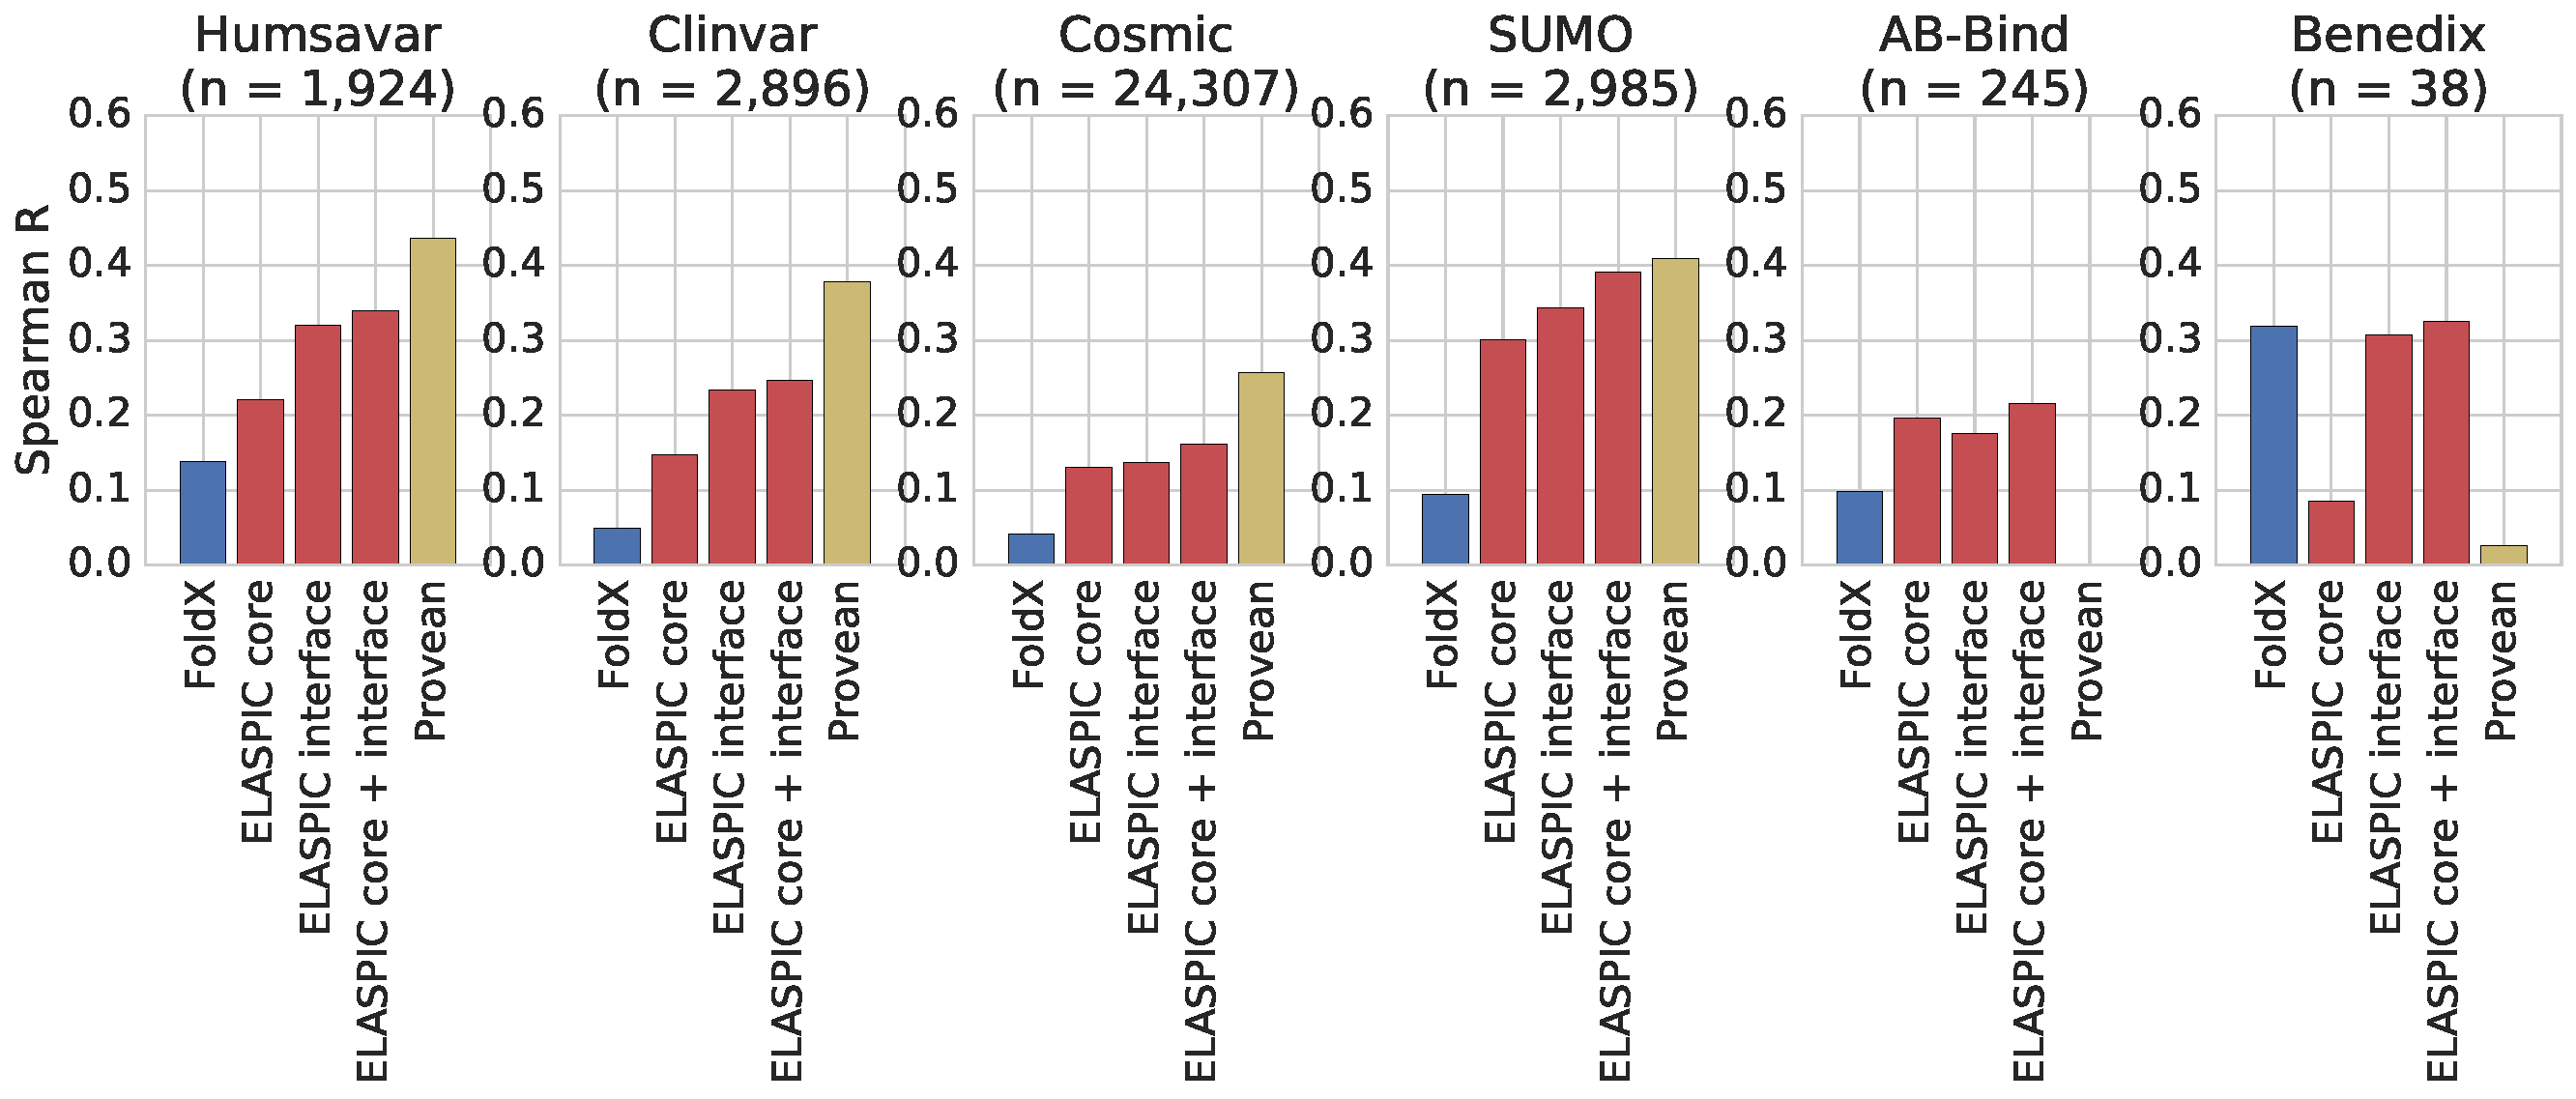
\includegraphics[width=1.0\textwidth]{static/elaspic_training_set/validation/test_performance_interface.pdf}
		\caption{Performance on the test datasets.}
		% \vspace*{10mm}
	\end{subfigure}

	\caption[Interface predictor validation.]{Performance of the interface predictor on the training (a), validation (b) and test sets (c).}
\end{figure}
